\section{Robustness}
The field measurements showed.
\cite{smolnik_5g_2020} \SI{3}{\metre} corn plants
Therefore, the following section focuses on the influence of the different physical layer parameters on the robustness of the IEEE 802.11ax standard
Wi-Fi transmissions.
\todo{Why Matlab? Why not ns-3?}
The MATLAB WLAN Toolbox \footnote{\url{https://de.mathworks.com/products/wlan.html?s_tid=AO_PR_info}} is a add-on to simulate, analyse, and test of wireless LAN communications systems.
The WLAN Toolbox supports a wide range of IEEE 802.11 standards.
Since Release R2019b \footnote{https://de.mathworks.com/help/wlan/release-notes.html}, the WLAN Toolbox supports the Signal Recovery, Packet Extension and Physical Layer abstractions to simulation IEEE 802.11ax networks.

My robustness analysis is based on the WLAN Toolbox example wlan/HESUExample \footnote{https://de.mathworks.com/help/wlan/ug/802-11ax-packet-error-rate-simulation-for-single-user-format.html} to simulate the \ac{PER} of point-to-point IEEE 802.11ax networks for
a specified \ac{SNR} values. \todo[color=yellow]{example?}

First, I set the IEEE 802.11ax physical layer parameters using the wlanHEConfig object, where I define the following default parameters:
\begin{itemize}
	\item \ac{GI} of \SI{3200}{\nano\second}
	\item \ac{BW} of \SI{20}{\mega\hertz}
	\item 2 spatial streams
	\item 2 transmit antennas
	\item \ac{DCM} disabled
	\item \ac{STBC} disabled
	\item \ac{LDPC} enabled
	\item HE-\ac{MCS} of 0
	\item \ac{CR} of 1/2
	\item Extended range mode disabled
\end{itemize}

Next, I chose a channel model to simulate the channel. The WLAN Toolbox supports a wide range of channel models, such as wlanTGaxChannel, wlanTGnChannel, wlanTGacChannel, and wlanTGnChannel.
The wlanTGaxChannel model supports six different channel models for IEEE 802.11ax networks, named TGax-A, TGax-B, TGax-C, TGax-D, TGax-E, and TGax-F.

As I want to simulate outdoor scenarios, I chose the TGax-F channel model, which is suitable for outdoor scenarios.
The wlanTGaxChannel model supports configuring the \ac{BW}, the number of transmit and receive antennas, which I set equal to the configuration of the wlanHEConfig object.
\cite{GermanLaw} allow outdoor transmission in the frequency range of \SI{5.725}{\giga\hertz} to \SI{5.825}{\giga\hertz}. Therefore, I set the carrier frequency to \SI{5.6}{\giga\hertz}.
Additional parameters are left at their default values as they are not relevant for outdoor scenarios.
\begin{figure}%
	\centering
	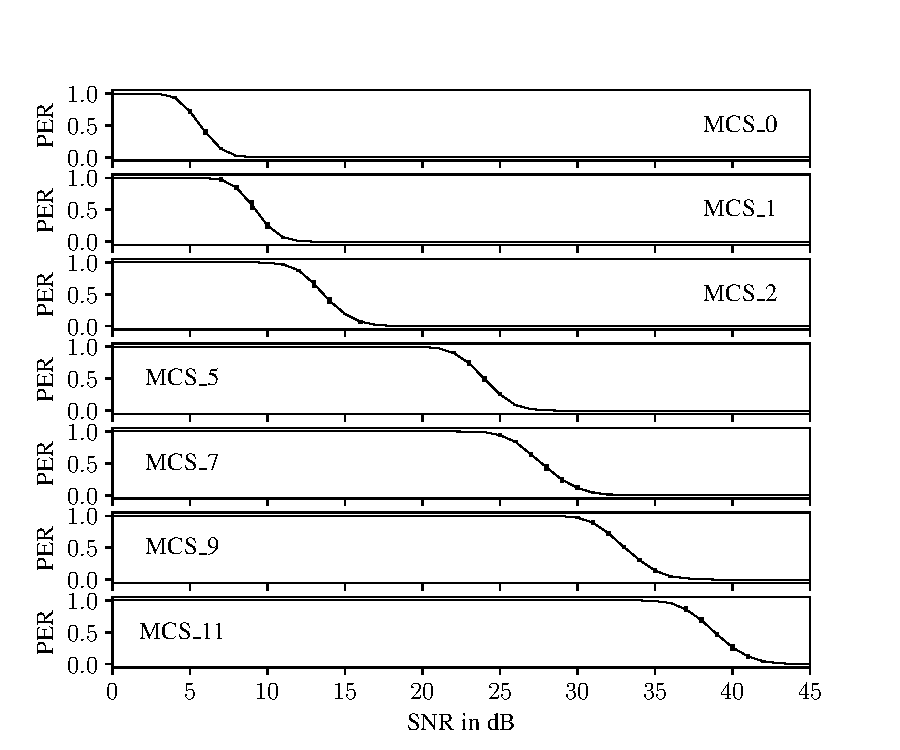
\includegraphics[width=0.95\textwidth]{figures/MCS_PER_to_SNR.pdf}
	\caption{Achieved Goodput and theoretical Datarate of two WiFi 6 stations in Ad-Hoc Mode with a \ac{GI} of \SI{3200}{\nano\second} and a bandwidth of \SI{40}{\mega\hertz} in regards to the number of the chosen \ac{MCS} and \ac{CR} and whether \ac{DCM} is enabled}%
	\label{fig:PER_SNR_MCS}%
\end{figure}


\begin{figure}%
	\centering
	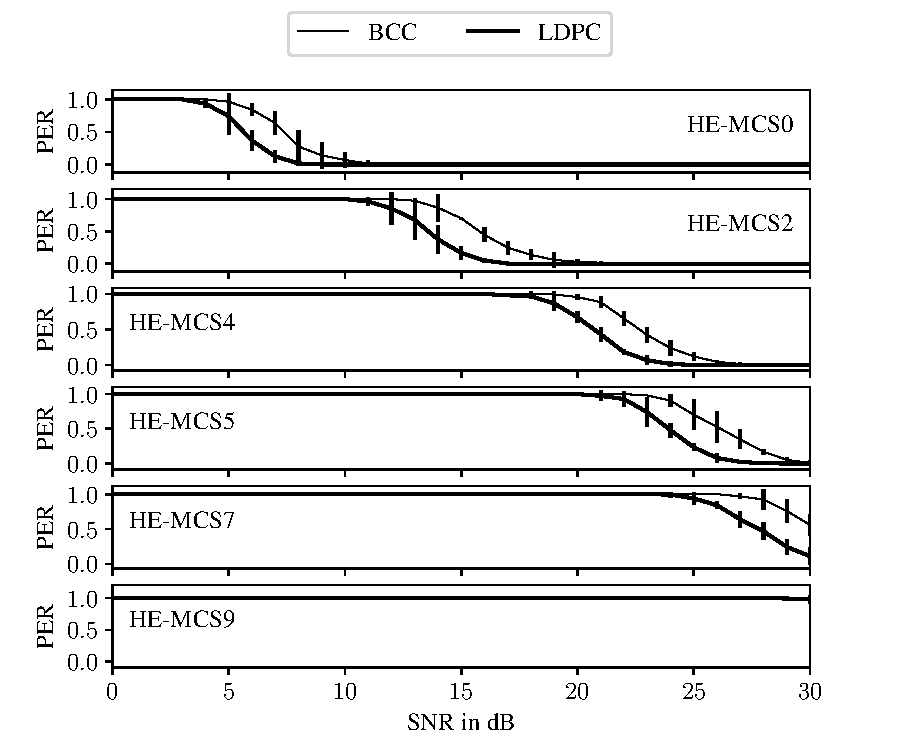
\includegraphics[width=0.95\textwidth]{figures/LDPC_PER_to_SNR.pdf}
	\caption{Simulated \ac{PER} in regards to \ac{SNR} for chosen HE-\ac{MCS} values and whether \ac{LDPC} or \ac{BCC} is enabled for IEEE 802.11ax physical layer parameters of a \ac{GI} of \SI{3200}{\nano\second}, a bandwidth of \SI{20}{\mega\hertz} and 2 spatial streams}%
	\label{fig:PER_SNR_LDPC}%
\end{figure}

\begin{figure}%
	\centering
	
\includegraphics[width=0.95\textwidth]{figures/GI_PER_to_SNR.pdf}
	\caption{Achieved Goodput and theoretical Datarate of two WiFi 6 stations in Ad-Hoc Mode with a \ac{GI} of \SI{3200}{\nano\second} and a bandwidth of \SI{40}{\mega\hertz} in regards to the number of the chosen \ac{MCS} and \ac{CR} and whether \ac{DCM} is enabled}%
	\label{fig:PER_SNR_GI}%
\end{figure}

\begin{figure}%
	\centering
	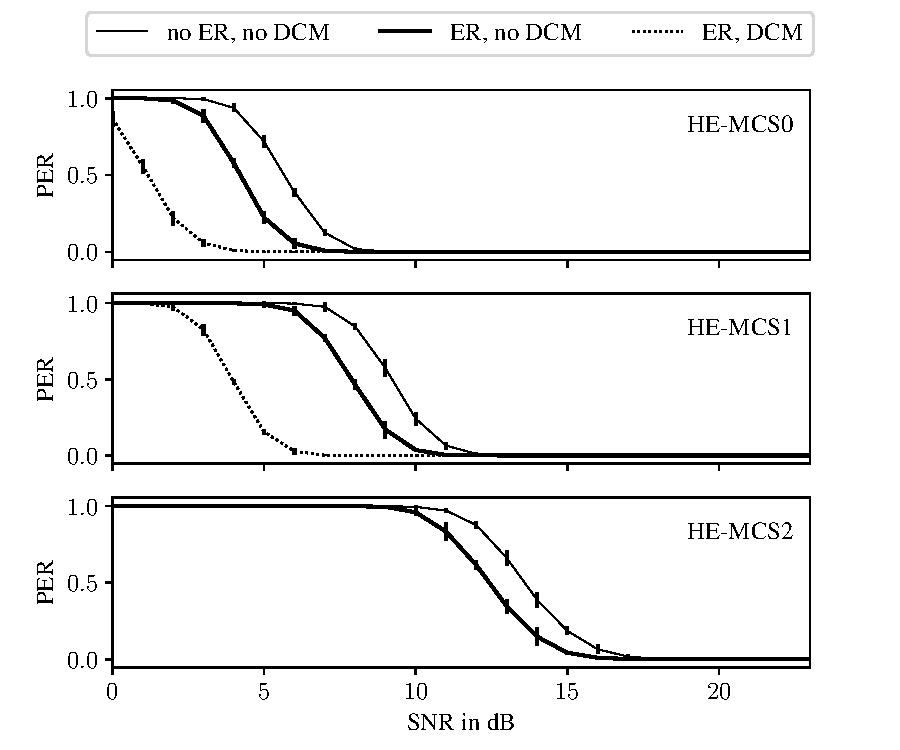
\includegraphics[width=0.95\textwidth]{figures/ER_PER_to_SNR.pdf}
	\caption{Simulated \ac{PER} in regards to \ac{SNR} for chosen HE-\ac{MCS} values and whether Extended Range or \ac{DCM}
	is enabled for IEEE 802.11ax physical layer parameters of a \ac{GI} of \SI{3200}{\nano\second}, a \ac{BW} of \SI{20}{\mega\hertz} and 2 spatial streams}
	\label{fig:PER_SNR_ER}%
\end{figure}

\begin{figure}%
	\centering
	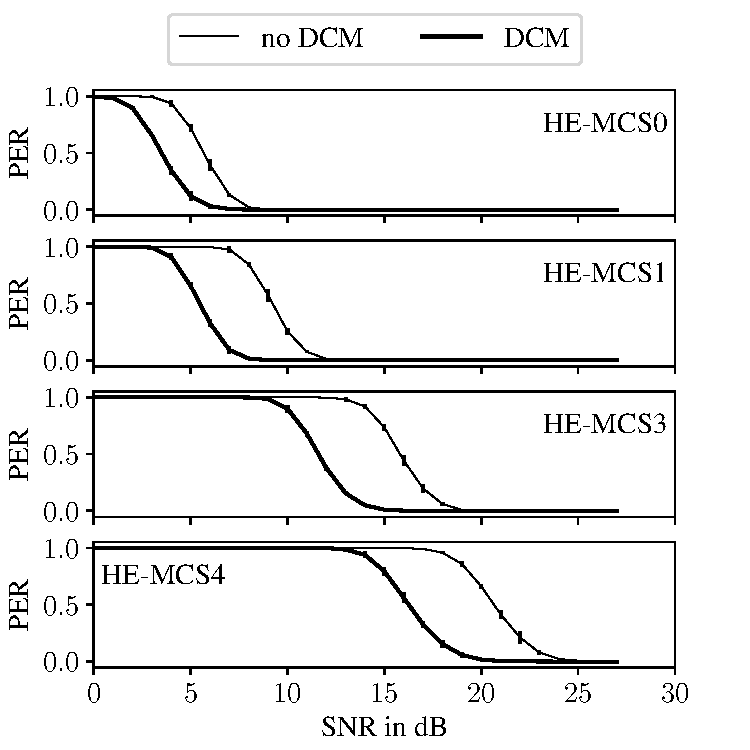
\includegraphics[width=0.95\textwidth]{figures/DCM_PER_to_SNR.pdf}
	\caption{Simulated \ac{PER} in regards to \ac{SNR} for chosen HE-\ac{MCS} values and whether \ac{DCM} is enabled for IEEE 802.11ax physical layer parameters of a \ac{GI} of \SI{3200}{\nano\second}, a \ac{BW} of \SI{20}{\mega\hertz} and 2 spatial streams}%
	\label{fig:PER_SNR_DCM}%
\end{figure}
no DCM, no ER

\begin{figure}%
	\centering
	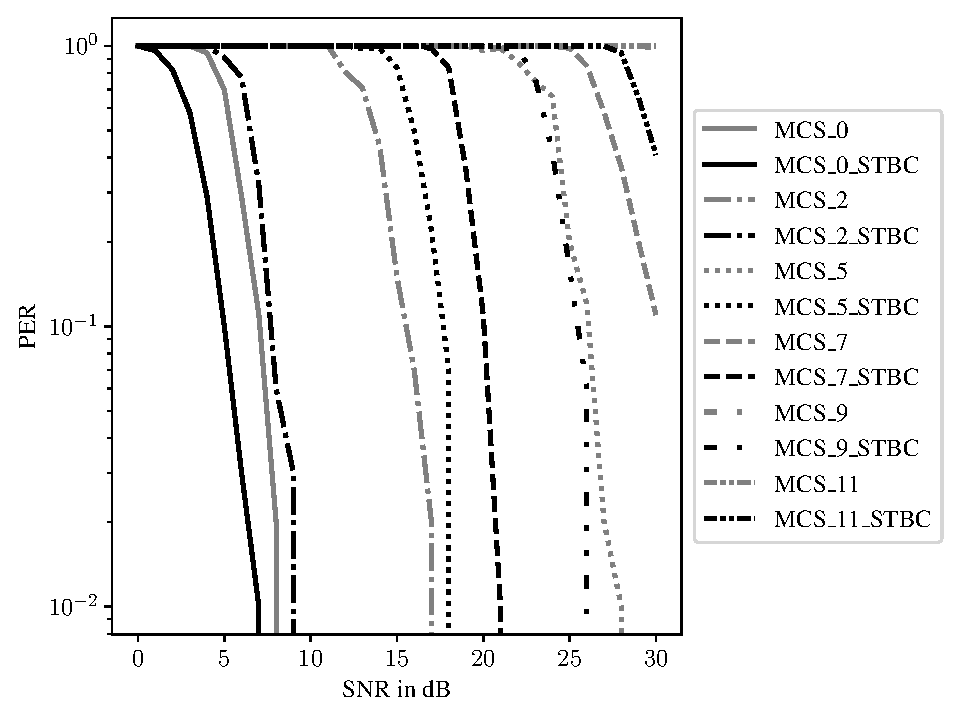
\includegraphics[width=0.95\textwidth]{figures/STBC_PER_to_SNR.pdf}
	\caption{Simulated \ac{PER} in regards to \ac{SNR} for chosen HE-\ac{MCS} values and whether \ac{STBC} is enabled for IEEE 802.11ax physical layer parameters of a \ac{GI} of \SI{3200}{\nano\second}, a \ac{BW} of \SI{20}{\mega\hertz} and 2 spatial streams}%
	\label{fig:PER_SNR_STBC}%
\end{figure}